\documentclass[letterpaper,11pt]{article}

\usepackage{latexsym}
\usepackage[empty]{fullpage}
\usepackage{titlesec}
\usepackage{marvosym}
\usepackage[usenames,dvipsnames]{color}
\usepackage{verbatim}
\usepackage{enumitem}
\usepackage[hidelinks]{hyperref}
\usepackage{fancyhdr}
\usepackage[english]{babel}
\usepackage{tabularx}
\usepackage{fontawesome5}
\usepackage{multicol}
\setlength{\multicolsep}{-3.0pt}
\setlength{\columnsep}{-1pt}
\input{glyphtounicode}

%new packages

\usepackage{fontenc}
\usepackage{amsmath}
\usepackage{amssymb}
\usepackage{graphicx}



%----------FONT OPTIONS----------

\pagestyle{fancy}
\fancyhf{} % clear all header and footer fields
\fancyfoot{}
\renewcommand{\headrulewidth}{0pt}
\renewcommand{\footrulewidth}{0pt}

% Adjust margins
\addtolength{\oddsidemargin}{-0.6in}
\addtolength{\evensidemargin}{-0.5in}
\addtolength{\textwidth}{1.19in}
\addtolength{\topmargin}{-.7in}
\addtolength{\textheight}{1.4in}

\urlstyle{same}

\raggedbottom
\raggedright
\setlength{\tabcolsep}{0in}

% Sections formatting
\titleformat{\section}{
  \vspace{-4pt}\scshape\raggedright\large\bfseries
}{}{0em}{}[\color{black}\titlerule \vspace{-5pt}]



% Ensure that generate pdf is machine readable/ATS parsable
\pdfgentounicode=1

%-------------------------
% Custom commands
\newcommand{\resumeItem}[1]{
  \item\small{
    {#1 \vspace{-2pt}}
  }
}

\newcommand{\classesList}[4]{
    \item\small{
        {#1 #2 #3 #4 \vspace{-2pt}}
  }
}

\newcommand{\resumeSubheading}[4]{
  \vspace{-2pt}\item
    \begin{tabular*}{1.0\textwidth}[t]{l@{\extracolsep{\fill}}r}
      \textbf{#1} & \textbf{\small #2} \\
      \textit{\small#3} & \textit{\small #4} \\
    \end{tabular*}\vspace{-7pt}
}

\newcommand{\resumeSubSubheading}[2]{
    \item
    \begin{tabular*}{0.97\textwidth}{l@{\extracolsep{\fill}}r}
      \textit{\small#1} & \textit{\small #2} \\
    \end{tabular*}\vspace{-7pt}
}

\newcommand{\resumeProjectHeading}[2]{
    \item
    \begin{tabular*}{1.001\textwidth}{l@{\extracolsep{\fill}}r}
      \small#1 & \textbf{\small #2}\\
    \end{tabular*}\vspace{-7pt}
}


\newcommand{\resumeSubItem}[1]{\resumeItem{#1}\vspace{-4pt}}

\renewcommand\labelitemi{$\vcenter{\hbox{\tiny$\bullet$}}$}
\renewcommand\labelitemii{$\vcenter{\hbox{\tiny$\bullet$}}$}

\newcommand{\resumeSubHeadingListStart}{\begin{itemize}[leftmargin=0.0in, label={}]}
\newcommand{\resumeSubHeadingListEnd}{\end{itemize}}
\newcommand{\resumeItemListStart}{\begin{itemize}}
\newcommand{\resumeItemListEnd}{\end{itemize}\vspace{-5pt}}

\begin{document}
\fontfamily{cmr}\selectfont
\begin{center}
\parbox{3.0cm}{%
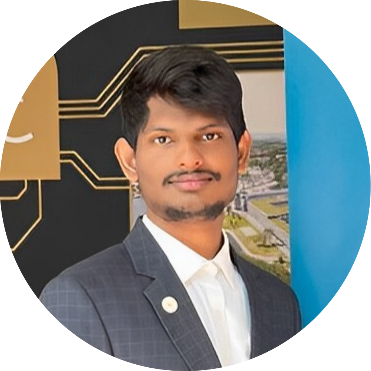
\includegraphics[width=2.7cm,clip]{images/resume_pic_m.png}}
}
\parbox{\dimexpr\linewidth-3.8cm\relax}{
\vspace{-20pt}
\begin{tabularx}{\linewidth}{L r} \\
    {\Huge \scshape  Venkata Sai Yakkshit Reddy Asodi}~
    \href{https://www.cedzlabs.com/yakkshit}{\vspace{1pt}}\\
      India. \\ \vspace{1pt}
     \small \raisebox{-0.1\height}\faPhone\ +91 8179936156 ~ \href{mailto:saiyakkshit2001@gmail.com}{\raisebox{-0.2\height}\faEnvelope\  {saiyakkshit2001@gmail.com}} ~ 
    \href{https://linkedin.com/in/yakkshit/}{\raisebox{-0.2\height}\faLinkedin\ {yakkshit}}  ~
    \href{https://yakkshit.com/}{\raisebox{-0.2\height}\faGlobe\ {yakkshit.com}}  ~
    \href{https://github.com/yakkshit}{\raisebox{-0.2\height}\faGithub{ yakkshit}}
    \vspace{-8pt}
    
\end{tabularx}
}
\end{center}

\vspace{-23pt}
\section{Summary}
Motivated Machine Learning Engineer with hands-on experience in developing AI-powered dashboards and deep learning models. Proficient in PyTorch, TensorFlow, and AWS services. Passionate about building scalable machine learning solutions and collaborating with research teams on innovative AI projects.

%-----------PROGRAMMING SKILLS-----------
\section{Technical Skills}
\begin{itemize}[leftmargin=0.15in, label={}]
\small{\item{
\textbf{Frameworks - }{PyTorch, TensorFlow, Streamlit, Scikit-learn} \\
\textbf{Languages - }{Python, JavaScript, SQL, Bash} \\
\textbf{Tools - }{AWS S3, EC2, Athena, Docker, Git} \\
\textbf{Deployment - }{AWS, MLOps, Docker, Kubernetes} \\
}}
\end{itemize}

%-----------EXPERIENCE-----------
\section{Experience}

\resumeSubheading
{Circleup AG}{January 2024 -- July 2024}
{Lead Full Stack Engineer}{Zurich, Switzerland}\\
\vspace{10pt}
\textbf{Responsibilities:}
\begin{itemize}[leftmargin=0.15in, label={}]
\item Collaborated with research scientists on deep learning models for AI-based customer support solutions using PyTorch and TensorFlow.
\item Developed and optimized ML models for large datasets using AWS S3 and EC2.
\item Created dashboards using Streamlit to visualize predictive analytics for internal projects.
\end{itemize}

\resumeSubheading
{Cedzlabs}{March 2023 -- December 2023}
{Full Stack Developer}{Remote, India}\\
\vspace{10pt}
\textbf{Responsibilities:}
\begin{itemize}[leftmargin=0.15in, label={}]
\item Built ML models for sentiment analysis and classification tasks using Scikit-learn and PyTorch.
\item Developed intuitive web-based dashboards for monitoring model performance and real-time data insights.
\end{itemize}

%-----------PROJECTS-----------
\section{Projects}

\resumeProjectHeading
{\textbf{AI Dashboard for Predictive Analytics} $|$ \emph{PyTorch, AWS S3, Streamlit}}{April 2024 -- July 2024}\\
\vspace{6pt}
\textbf{Description:}
\begin{itemize}[leftmargin=0.15in, label={}]
\item Developed a dashboard using Streamlit to visualize and monitor predictive models trained on large datasets.
\item Integrated AWS S3 for data storage and EC2 for high-performance model training.
\end{itemize}

\resumeProjectHeading
{\textbf{Deep Learning Model Deployment on AWS} $|$ \emph{TensorFlow, Docker, EC2}}{August 2023 -- December 2023} \\
\vspace{6pt}
\textbf{Description:}
\begin{itemize}[leftmargin=0.15in, label={}]
\item Created scalable model training pipelines on AWS EC2 using Docker and TensorFlow.
\item Deployed MLOps solutions to automate model retraining and monitoring.
\end{itemize}

%-----------ACHIEVEMENTS-----------
\section{Achievements}
\begin{itemize}[leftmargin=0.15in, label={}]
\item Deployed and optimized deep learning models for large datasets on AWS cloud.
\item Active contributor to open-source projects related to machine learning and AI.
\item Participated in tech conferences and meetups focusing on AI innovations.
\end{itemize}

\section*{Languages}
\begin{itemize}
  \item Telugu - Native $|$ English - Fluent $|$ Hindi - Fluent $|$ German - Elementary.
\end{itemize}

\end{document}